\section{Results}
This section describes the results of the interview study. First, a brief overview of the sample will be given. Then, the findings will be discussed, separated by motivational factors and factors that hindered the participants from effectively using and interpreting the charts. The final category system of the study is shown in Figure \ref{fig:category_system}.

\begin{figure}[htb!]
    \centering
    \fbox{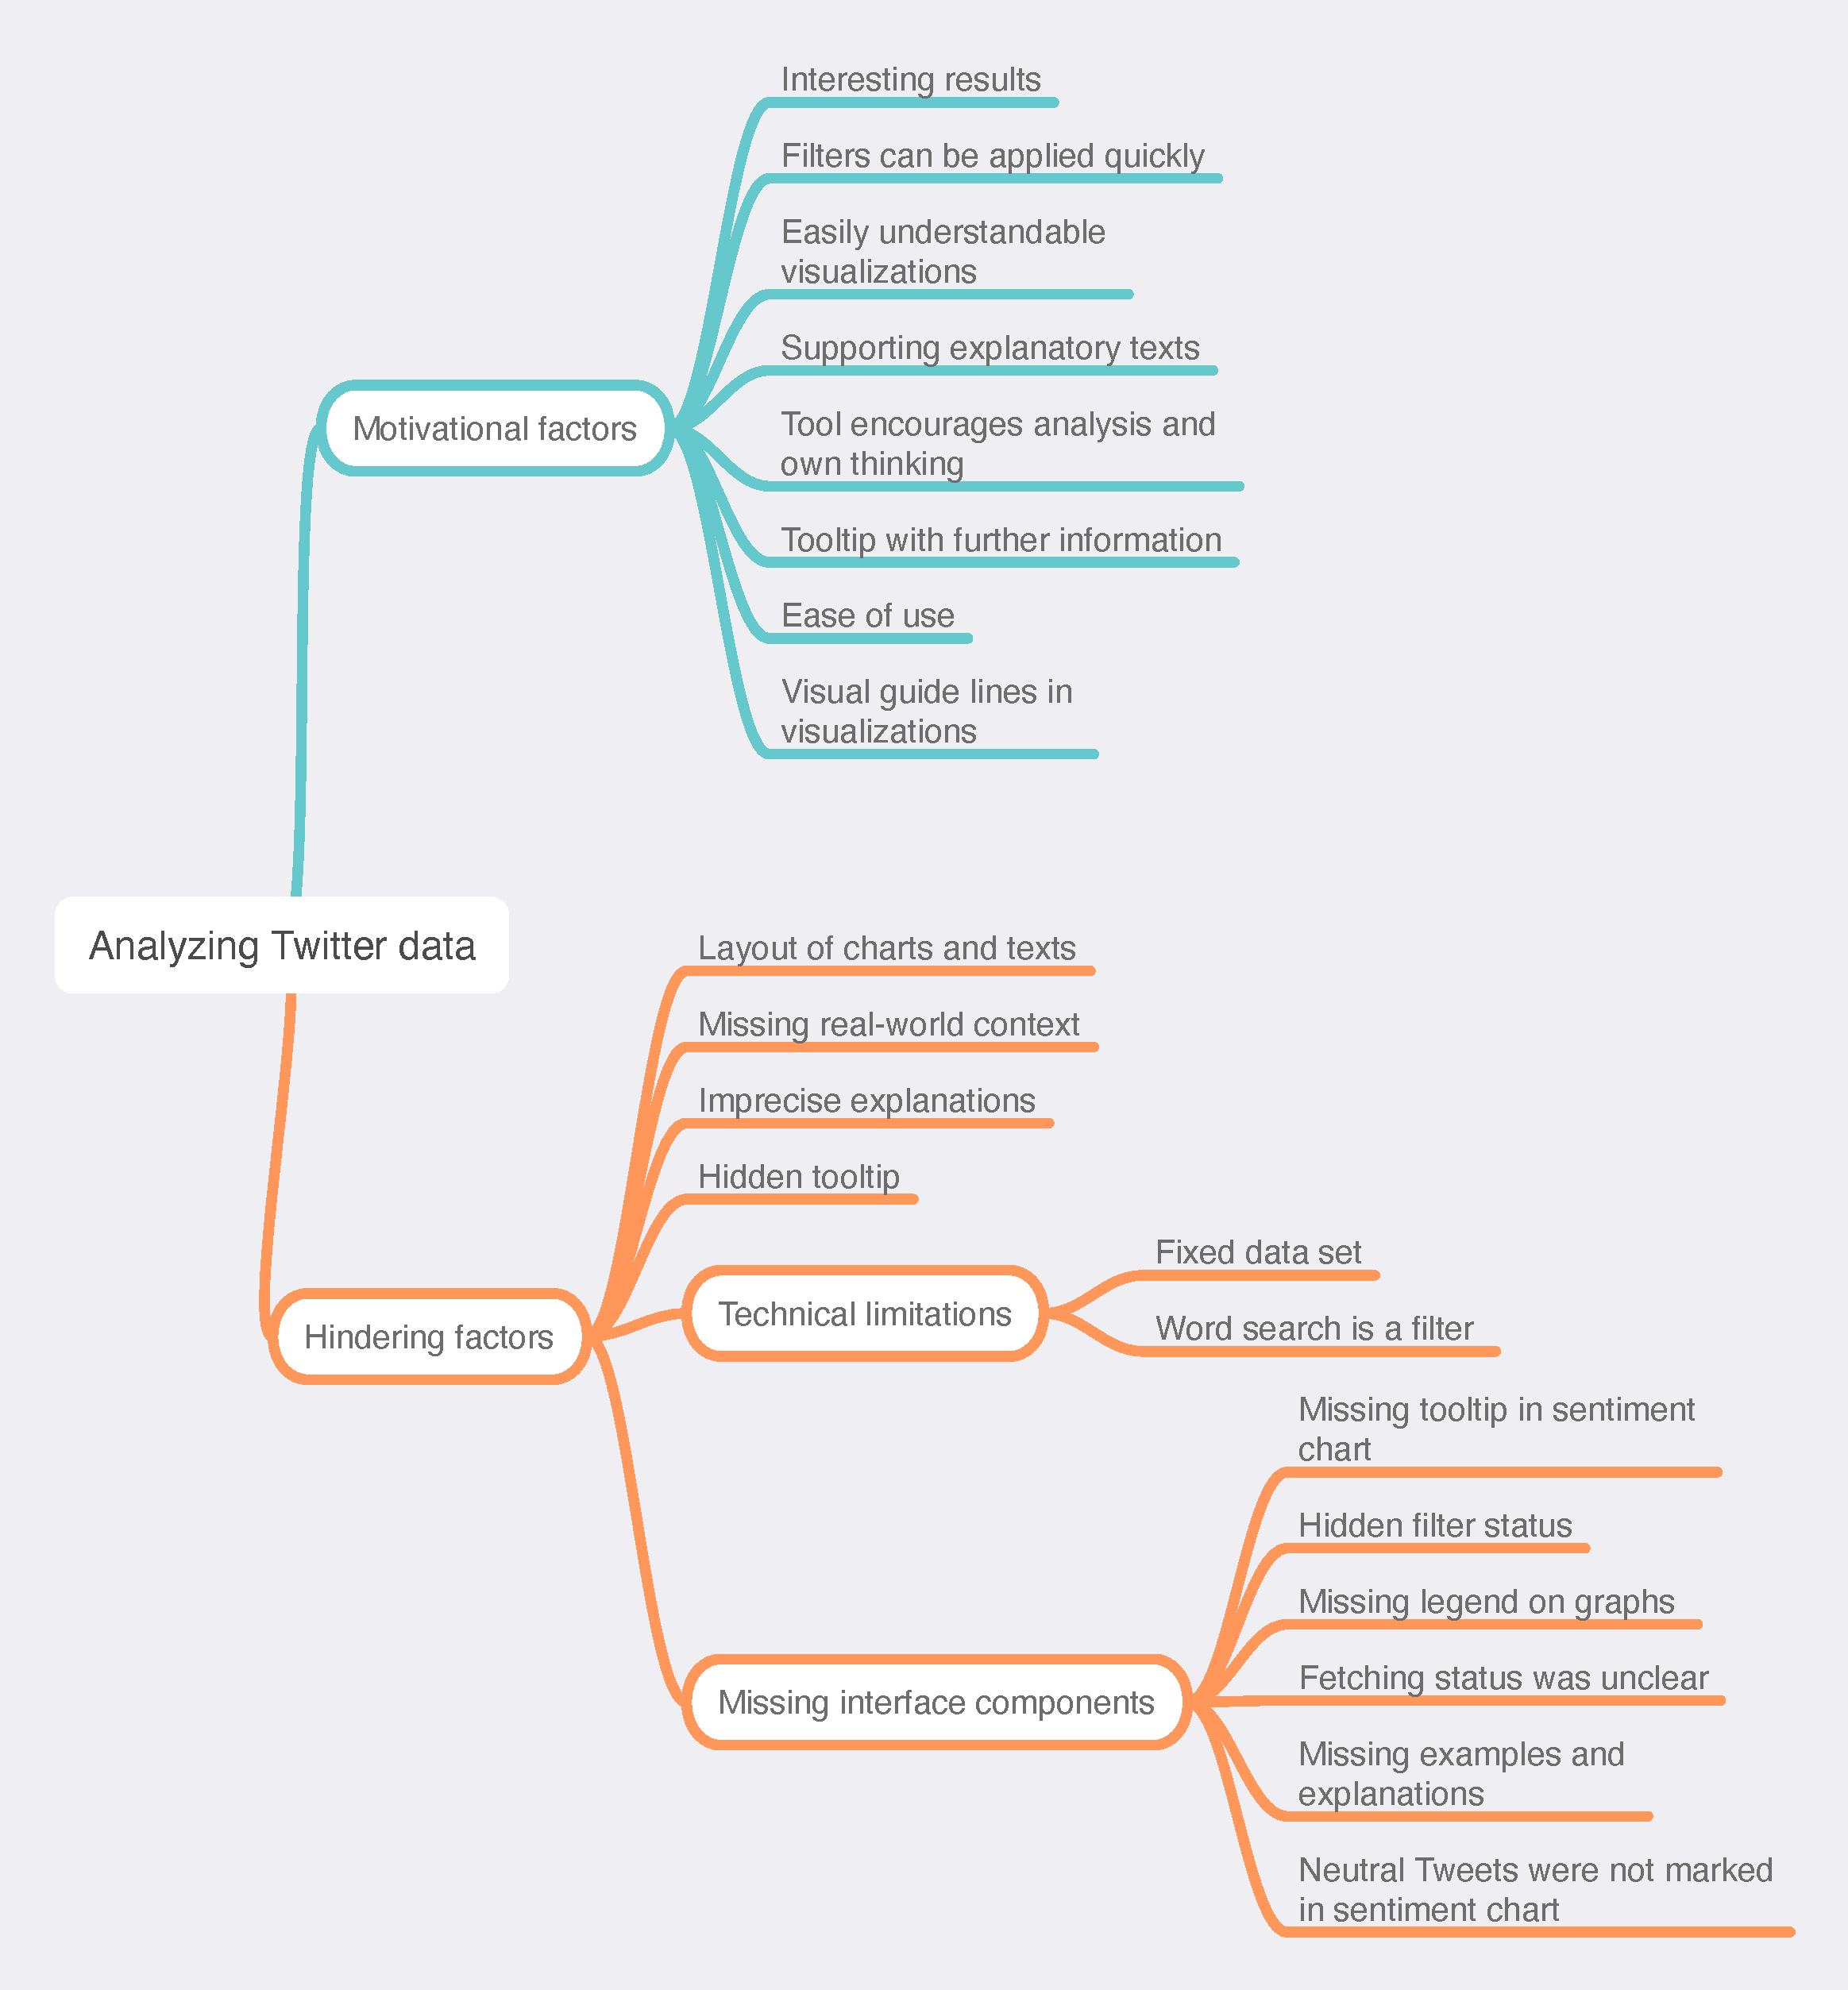
\includegraphics[width=\linewidth]{images/category_system.pdf}}
    \caption{The final category system.}
    \label{fig:category_system}
\end{figure}

\subsection{Sample description}
For the qualitative user study, six participants between the age of 23 and 26 were recruited. The study was limited to six participants because studies have shown that five to six user tests already uncover around 80\% of usability problems (\cite{10.1145/169059.169166}).

%TODO: grafische Aufbereitung der Ergebnisse des Screening-Fragebogens?

3 participants identify themselves as male, 3 participants as female. The participants were chosen because they have little to no knowledge of big data and data visualization. This qualifies them as \emph{laymen}, the target group of this study.

Participants were asked to rate their interaction levels with twitter on a 6-point Likert scale from 1–never to 6–daily.

Twitter usage varied between the participants. 3 of them browse content on Twitter daily, 1 person at least a few times a week. 1 Participant never reads content on Twitter itself. All of the participants see twitter content at least sometimes on other web platforms. 5 participants rarely or never interact with content on Twitter, like using the like- or retweet button. The participants rarely post content on Twitter themselves.

\subsection{Motivational factors}
Motivational factors were factors that motivated participants to use the dashboard, explore the data set, and analyze the results. 9 motivational factors were identified in total which will be described in the following, along with anchor examples.

\subsubsection*{Interesting results}
Participants reported that they found the results they gathered from the visualizations interesting. One example is a participant who found it interesting that retweets make up most of the activity on Twitter:

\begin{quote}
    Aber schon spannend eigentlich, dass alles... also viele hauptsächlich Retweets sind und nicht eigene Tweets. (m23, l. 18)
\end{quote}

Others found the impact of retweets on the overall sentiment interesting:

\begin{quote}
    Ich fands sehr interessant zu sehen, wie so Retweets die Stimmung beeinflussen. (w25, l. 80)
\end{quote}

Participants also expressed that they liked to have the ability to see how a certain topic was discussed by the German Twitter-sphere:

\begin{quote}
    Aber ja, das ist schon interessant da mal nen Begriff reinzutippen und zu gucken, was passiert. (m24, l. 82)
\end{quote}

Some participants said that it was nice to see their own gut-feeling being backed by data:

\begin{quote}
    Ich finds sehr interessant zu sehen, wie so Retweets die Stimmung beeinflussen. Weil wenn man selbst Twitter benutzt merkt man halt auch selbst [...] dass mich persönlich das aufregt. Und das ist eigentlich sehr interessant gewesen zu sehen, dass das nicht nur mein Empfinden ist, sondern dass sich das generell in Twitter wiederfindet. Dass die Stimmung durch immer-wiederholen des gleichen Themas beeinflusst wird. (w25, l. 80)
\end{quote}

\subsubsection*{Filters can be applied quickly}
During testing, all participants used the toggles to show and hide retweets and neutral tweets multiple times in a row. This was likely done to compare the impact of retweets and neutral tweets on the data set.

\begin{quote}
    B: Und jetzt kann ich ja mal gucken wie sich das ändert, wenn ich die Retweets ausblende

    Screen: blendet die Retweets wiederholt aus und wieder ein (w26a, ll. 73-74)
\end{quote}

This behavior occured both during the free exploration and the task-solving phase of the interview.

\subsubsection*{Easily understandable visualizations}
Especially the bar chart which showed the tweet volume per day seemed to be easy to read for participants. This led to a quicker understanding of the data set and made it easier for participants to verify their assumptions. This participant, for example, wanted to see if a real-life event she knew of was reflected in the data set during free exploration:

\begin{quote}
    B: Ich probier es mal mit "Stuttgart", denn da gab es ja glaub ich eine der ersten dieser Hygiene-Demos
    
    Screen: gelbe Balken werden zwischen dem 21. und dem 24. Juni sichtbar
    
    B: Ah ja interessant, dann war diese Demo bestimmt am 21. Juni. Interessant. (w26b, ll. 6-8)
\end{quote}

Another participant explicitly said that both visualizations were easily understandable, even without further explanation:

\begin{quote}
    Und die Beschriftung der Achsen war auch so eindeutig, dass man... wahrscheinlich hätte ich da nicht einmal den Infotext gebraucht und die Grafiken hätten gereicht. (m26, l. 83)
\end{quote}

\subsubsection*{Supporting explanatory texts}
Participants reported that the explanatory texts that accompanied the visualizations were helpful. They aided them both in the exploration phase:

\begin{quote}
    Ich hab mich gerade kurz gefragt, was neutrale Tweets sind, aber hier unten steht ja die Erklärung dazu. (m26, l. 22)
\end{quote}

as well as while solving the tasks:

\begin{quote}
    I: Wie leicht ist es dir gefallen, die Aufgaben zu beantworten?

    B: Also ich würde sagen ziemlich leicht [...] Mit den Erklärungen fand ich die schon gut zu lösen. (w26b, ll. 68-69)
\end{quote}

\subsubsection*{Tool encourages analysis and own thinking}
Another point that participants liked was that the visualizations encouraged them to think about the meaning for themselves. One participant expressed joy that the interactive visualizations helped her answering questions she had on her own:

\begin{quote}
    Ne es gab ja so unendlich viele Corona-Visualisierungen immer. Und ich find das ganz cool, dass man hier sehr offen sich das anschauen kann. Weil sonst geben so Visualisierungen ja ziemlich genau vor, was man überhaupt sehen kann. (w26b, l. 63)
\end{quote}

Another participant liked that the tasks asked them to reflect on what they could read from the visualizations:

\begin{quote}
    Ja gerade jetzt die letzte Aufgabe war ja sehr interessant, fand ich. Das mal so zu sehen, dass das... ne also wenn man mal so drüber nachdenkt, den Effekt dann auch ein bisschen zu verstehen. (m24, l. 82)
\end{quote}

\subsubsection*{Tooltip with further information}
As discussed in the section \ref{sec:cutForTime}, the tooltip could only be realized in the graph that showed the tweet volume over time. This tooltip helped participants to explore the data set more efficiently:

\begin{quote}
    Screen: Hovert mit dem Mauszeiger über den längsten Balken
    B: Oh, gibt's hier... ne, doch, am 16.6. Ich hatte das eben gar nicht entdeckt, dass es nen Tooltip gibt, wenn man drüber hovert. Sonst hätte ich jetzt hier noch angefangen, die Tage abzuzählen. (m24, ll. 45-47)
\end{quote}

\subsubsection*{Ease of use}
This category contains statements from the participants where they expressed the ease of use of the visualizations. One participant said that she knew where to find which function after she saw the different parts of the interface once:

\begin{quote}
    Ich finde das sehr übersichtlich und eigentlich auch, wenn man sich das einmal angeschaut hat und einmal was wo find ich was, wo kann ich welche Daten aus- und wieder einblenden, schnell und gut benutzbar. Auch wenn man eigentlich nicht so ein Computer-Spezialist ist kann man doch sehr gut damit arbeiten. (w25, l. 78)
\end{quote}

Another participant said she was able to learn more about the way Twitter works in the prototype than on Twitter itself because the tool was easy to use:

\begin{quote}
    Aber prinzipiell ist das ziemlich cool und auch intuitiv. Also man kann ja selbst über diese Twittersuche sich relativ viele Daten selbst ziehen, aber das würdest du ja nicht machen wenn du da nicht selber so direkt mit rumspielen kannst. (w26b, l. 63)
\end{quote}

\subsubsection*{Guide lines in visualization}
Some participants voiced the usefulness of the guideline marking the 0-line in the line graph showing the sentiment (see \textbf{Figure \ref{fig:sentiment_drosten_noneutral}):}

\begin{quote}
    Ich würde sagen, also die Linie bewegt sich schon im Durchschnitt oberhalb des 0-Wertes hier, aber hier an manchen Tagen reißt sie deutlich nach unten ein. (w26a, l. 66)
\end{quote}

\clearpage
\subsection{Hindering factors}
Hindering factors are factors that hindered the participants in their usage of the tool in one way or another. These factors will be further examined and explained in the following section.

\subsubsection*{Hidden filter status}
Participants had trouble recognizing that the search word had an impact on both graphs.

\begin{quote}
    Achso, das gesuchte Wort ist immer noch Covid hier in dem Graph, oder? Ah, okay. (m23, l. 20)
\end{quote}

Other participants were unsure whether the retweet- and neutral tweet filters which were situated between the two visualizations had, in fact, an influence on the second visualization as well.

\begin{quote}
    Screen: Blendet die neutralen Tweets aus und scrollt zum Sentiment-Graph

    B: Eeehm... Moment, hat das hier nen Einfluss drauf?

    Screen: Togglet die neutralen Tweets nochmal an und aus

    B: Ah ja, hat es. (m24, ll. 58-61)
\end{quote}

Participants also reported that they forgot about the status of the filters while they were analyzing the visualizations:

\begin{quote}
    Und dann achtet man halt nicht auf solche Häkchen, die man irgendwie setzen kann, die sich dann auf alles auswirken. (w26b, l. 63)
\end{quote}

One participant also said that having to constantly scroll up to the filter status hindered her to effectively solve the tasks:

\begin{quote}
    Also es war eher die Frage, wie interpretiere ich das jetzt, welche Aussage kann ich aus dem, was ich da sehe, treffen. Und dann immer gucken "hab ich die jetzt eingeblendet, hab ich die jetzt ausgeblendet?", also da musste ich schon nen Moment länger drüber nachdenken. (w26a, l. 89)
\end{quote}

\subsubsection*{Missing legend on graphs}
Legends are used in color-coded graphs so that users can map the used colors to their meaning. An example of this can be seen in \textbf{Figure \ref{fig:legend_example}}.

\begin{figure}[h!tb]
    \centering
    \fbox{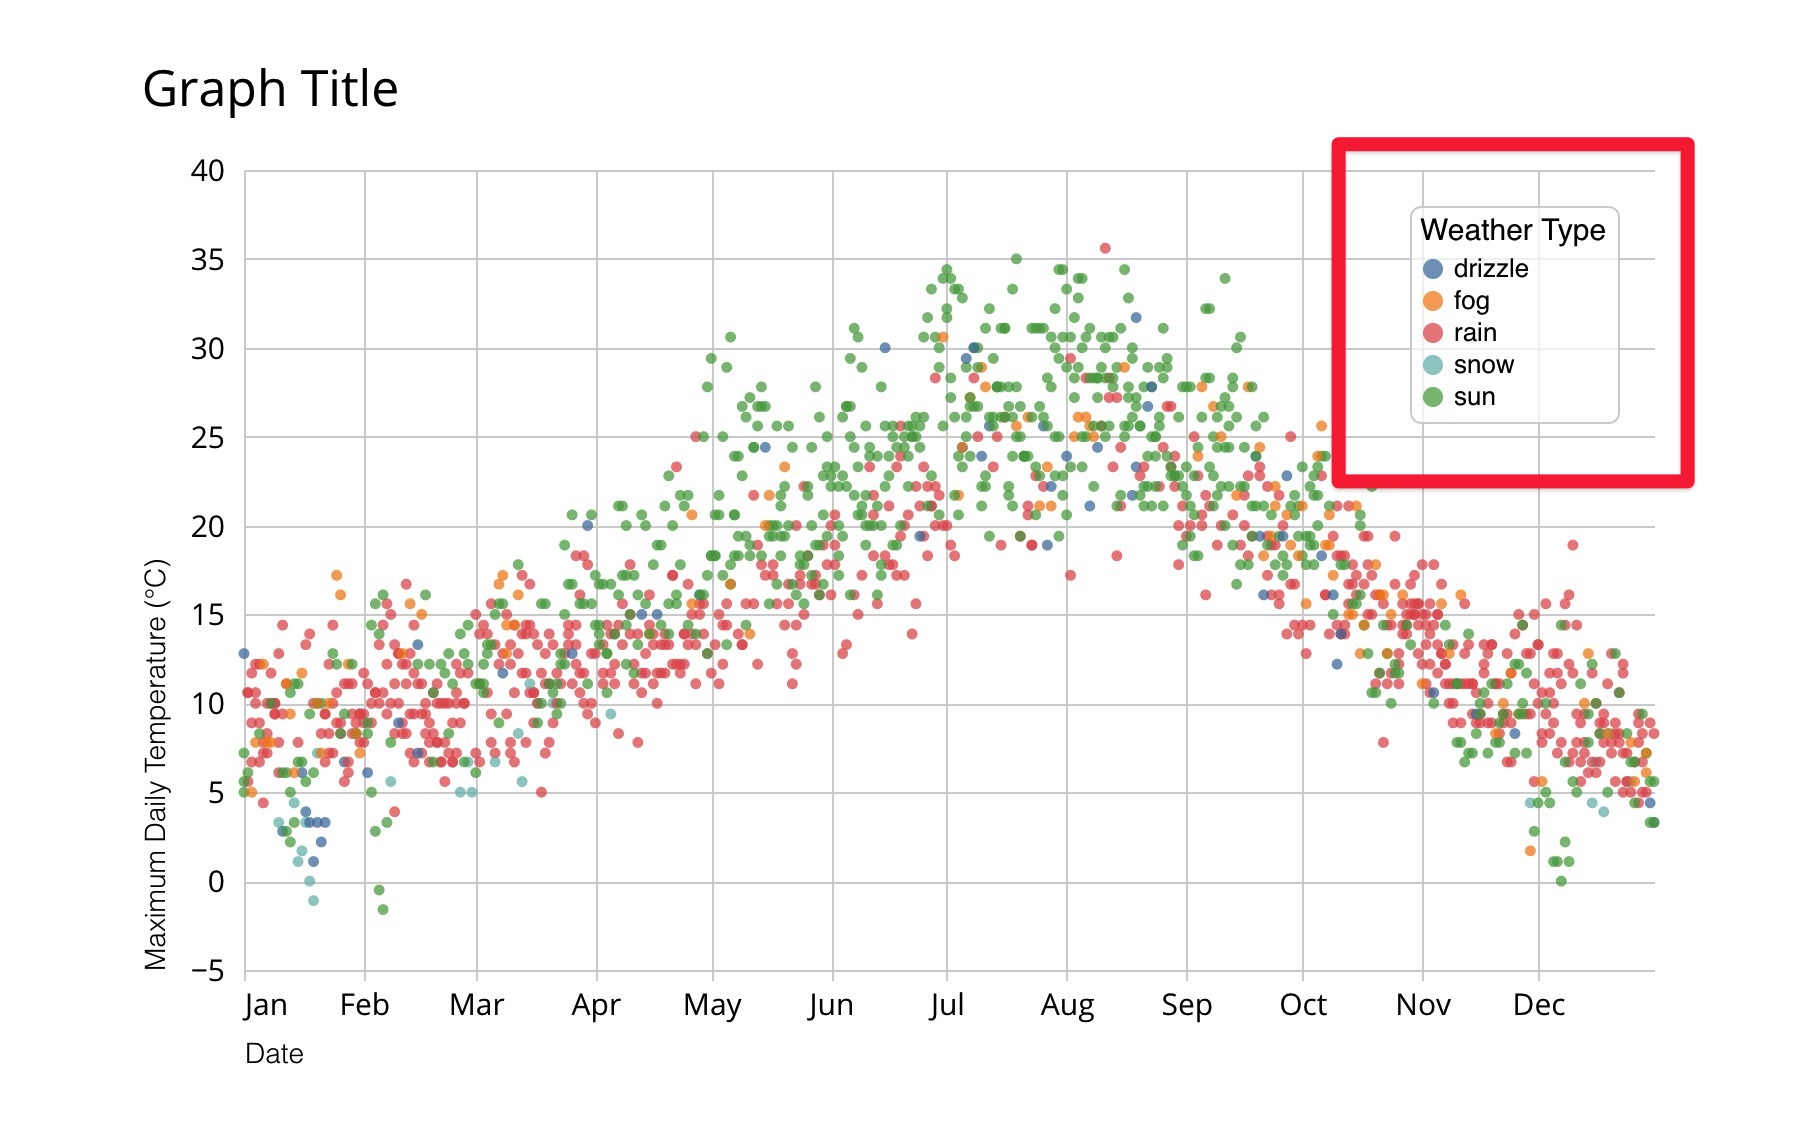
\includegraphics[width=0.7\linewidth]{images/legend_example.jpg}}
    \caption{Example of a legend. Screenshot from https://observablehq.com/@cahaber/cartesian-legend, highlight by the author}
    \label{fig:legend_example}
\end{figure}

The prototype did not have such a legend. Instead, the meaning of the different colors was explained in explanatory texts. Due to Observable using a notebook structure, These texts could not be placed next to the chart and thus had to be placed either below or above it. In this prototype, the chart was followed by its explanation.%, as seen in figure \ref{fig:sentiment_nolegend}.

% TODO: will ich die Grafik drin lassen? Evtl. um Platz zu schinden.
% \begin{figure}[h!tb]
%     \fbox{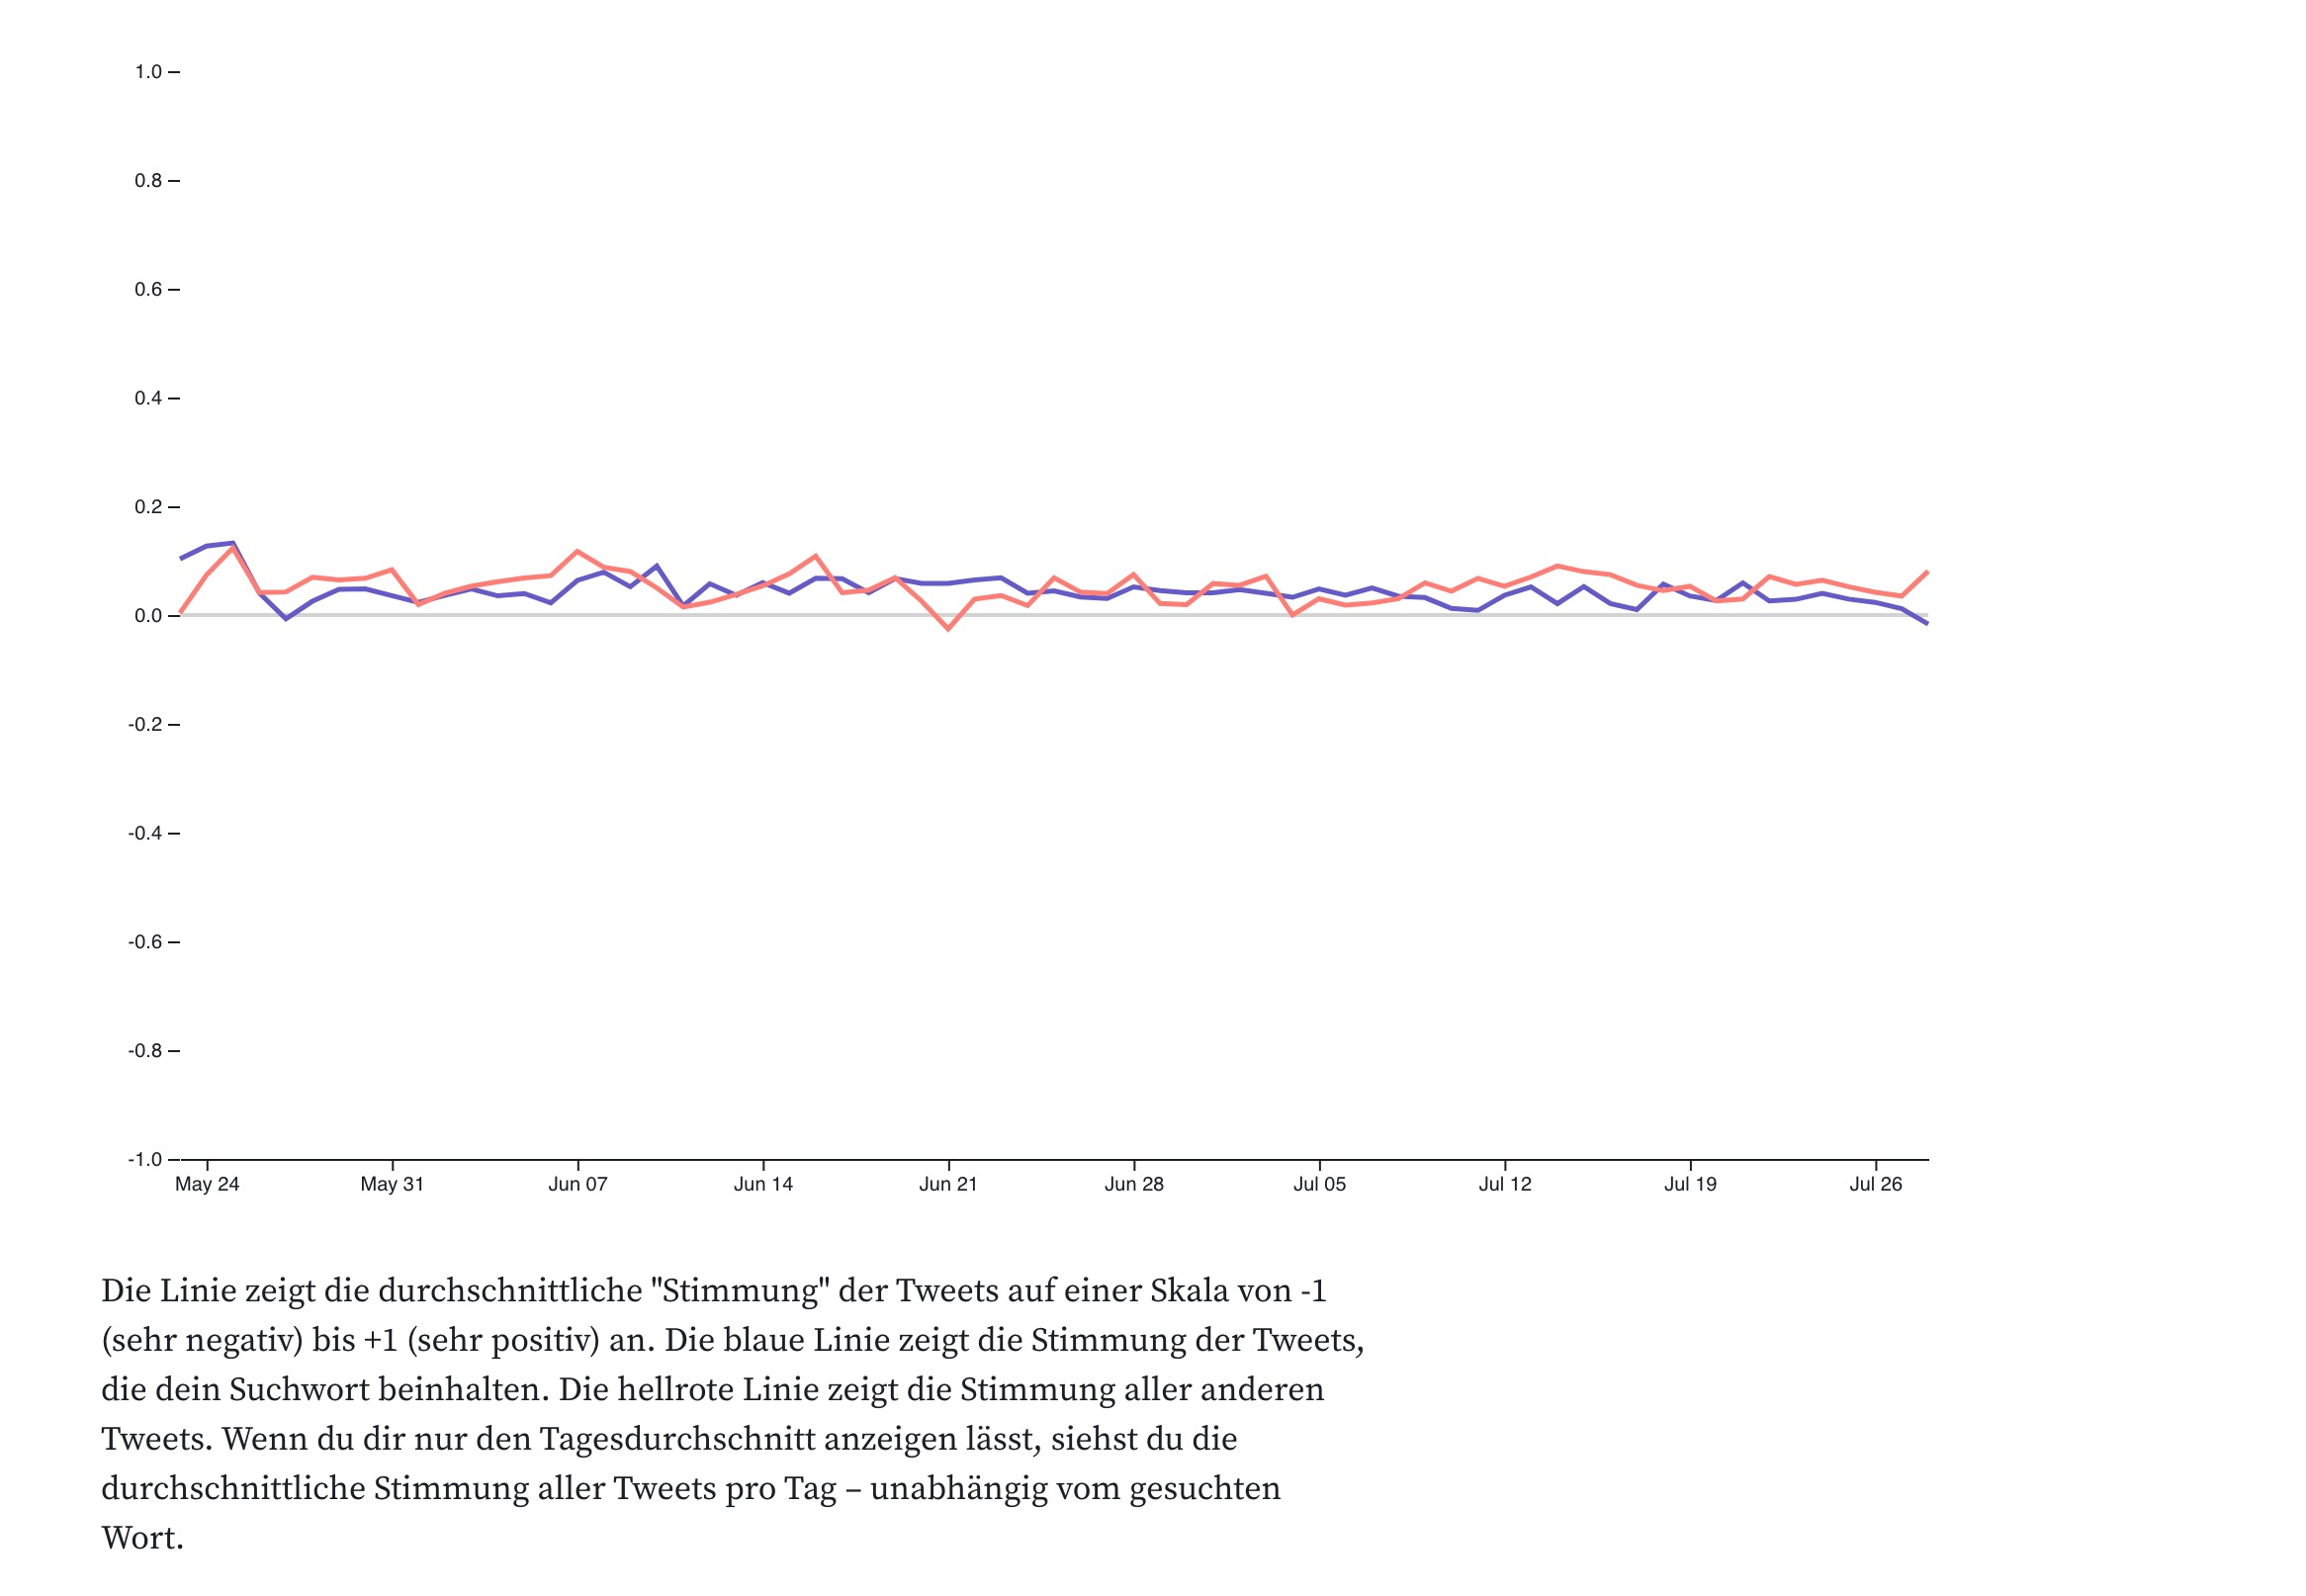
\includegraphics[width=\linewidth]{images/sentiment_nolegend.jpg}}
%     \caption{The sentiment chart with textual explanation of the colors below it}
%     \label{fig:sentiment_nolegend}
% \end{figure}

This resulted in several issues. One participant did not understand the meaning of the differently colored bars in the bar chart because she did not read the explanatory text thoroughly enough:

\begin{quote}
    B: Meine Frage ist jetzt nur, was bedeutet Orange und was bedeutet blau? 

    Screen: Scrollt etwas runter

    B: Da weiß ich aber nicht, ob das nachher noch kommt. Aber jetzt im ersten Moment hab ich nicht gesehen, was das bedeutet. (w25, ll. 8-10)
\end{quote}

The same participant had trouble recognizing the textually explained color in the sentiment chart.

\begin{quote}
    Screen: Scrollt zum Sentiment-Erklärtext runter

    B: Hä, rot? Ich seh gar keine hellrote Linie, sondern nur hier das Orange und blau.

    I: Ja, die orange Linie ist damit gemeint.

    B: Achso, okay. (w25, ll. 24-27)
\end{quote}

Another participant got confused by the textual explanation of the different parts of the chart. In this case, the word \say{blue} could have meant two different lines, one dark blue and one light blue.

\begin{quote}
    "Die Linie zeigt die durchschnittliche Stimmung..." Aber welche Linie ist denn jetzt DIE Linie? Dann gibt es eine blaue und eine hellblaue. (m24, l. 65)
\end{quote}

\subsubsection*{Layout of charts and texts}
This category contains problems that arose during testing that stem from the layout of charts and texts. One participant did not see the explanatory text for the sentiment graph as it was below the graph itself:

\begin{quote}
    B: Okay, ich glaub ich hab noch nicht ganz verstanden, was mir der Graph sagen will. Also, Sentiment ist quasi die Wertung?

    I: weiter unten steht auch noch mehr Erklärtext dazu.

    B: Okay. Aaah okay, das ist der Text hier unten (m23, ll. 22-24)
\end{quote}

Another participant seemed to be confused by the sentiment chart. After he found the explanatory text below the chart, he could continue with the task.

\begin{quote}
    Screen: Scrollt wieder zum Sentiment-Graphen runter
    
    B: Ach aber auch hier kein besonders überraschendes Sentiment. Warte, was... was tut denn hier die blaue?

    Screen: Fährt mit dem Cursor über den Erklärtext unter dem Graphen
    
    B: Ah, okay. Joar, okay. Dann... vielleicht doch eher. (m24, ll. 28-31) 
\end{quote}

One participant explicitly stated that he would have preferred to have the explanation texts \emph{above} the charts.

\begin{quote}
    Ich glaub das einzige, was ich gemacht hätte, wäre, den Infotext über die Grafik zu packen. Das wär für mich praktischer gewesen, weil dann lese ich erst, was ich sehe, und sehe dann erst die Grafik. Wobei ich jetzt gerade auch nen relativ kleinen Bildschirm habe. (m26, l. 75)
\end{quote}

However, one participant who studies to become a teacher said that she liked the layout from a pedagogical perspective.

\begin{quote}
    I: Das heißt, für deinen Lesefluss und das Verständnis wäre es besser gewesen, wenn du den Erklärtext über der Darstellung hast, die erklärt wird?

    B: Das ist ne gute Frage, also ich glaube aus einer verständnistheoretischen Perspektive ist es wahrscheinlich schlauer, wenn man sich erst die Frage stellt, bisschen irritiert ist und dann die Antwort findet und dann das versteht. Wenn man es erst liest und nicht genau weiß, worauf sich das jetzt bezieht, muss man den Text im Zweifelsfall zwei Mal lesen. Weil dann liest du das halt, denkst "hä?", dann schaust du dir das an und merkst dann, dass du Informationen dazu bekommen hast. Und dann liest du dir das nochmal durch. (w26a, ll. 80-81)
\end{quote}

\subsubsection*{Word search is a filter}
This category contains statements where the participants stumbled over the limitations of the word filter. The word filter filters for exact matches of the entered term in the database. This is a difference to search engines like Google or DuckDuckGo: these engines use a so-called \emph{fuzzy search}, which means that results do not only contain the exact search term, but also similar terms.

One participant entered a too specific keyword, but could quickly recover from this:

\begin{quote}
    Screen: Gibt "Dr. Drosten" in den Suchfilter ein

    B: Dann würd ich eben erst mal Dr. Drosten in diese Suchleiste hier oben eingeben

    Screen: wenige Ergebnisse werden gezeigt

    B: Wobei vielleicht geb ich besser nur "Drosten" ein weil den Doktor... filtern die Leute ja wahrscheinlich raus. (w26b, ll. 37-40)
\end{quote}

Another participant made a spelling mistake when filtering for a word which she did not recognize until she was made aware of it:

\begin{quote}
    Screen: Gibt im Wortfilter "Tonnies" ein, es werden nur sehr wenige Ergebnisse angezeigt

    B: Hm, jetzt seh ich hier gar nix

    I: Du hast Tönnies falsch geschrieben. Mit O statt mit Ö.
    
    B: Aah, I see. 

    Screen: Gibt Tönnies ein

    B: Okay, und verändert sich jetzt was? Ah ja, okay!  (w26a, ll. 10-15)
\end{quote}

Without the author's intervention, this participant most likely would not have been able to recover from her mistake, thinking that \emph{Tönnies} did not appear in the set of collected tweets.

\subsubsection*{Missing real-world context}
While the participants were able to identify days with high activity for a specific topic, the dashboard did not offer more information about what happened on that day. Some participants said that they could have used this information to interpret the findings better.

\begin{quote}
    B: Ganz witzig, am 5. und am 19. Juli gibts hier so... wie nennt man das denn, kein Peak sondern das Gegenteil  eines Peaks wo es dann so krass runtergeht. Das wäre interessant zu wissen, was an diesen Tagen war, ob die Leute da wohl schlechter drauf waren in Bezug auf Corona.  (w26b, l. 18)
\end{quote}

\subsubsection*{Fetching status was unclear}
When the word filter is changed, new data is fetched from the database. This means that it takes about five seconds between typing in a new search word and the results for this word being displayed. Participants felt unsure about whether their input had already been processed or if they have to wait a bit longer, as the fetching status was not shown in the interface.

\begin{quote}
    B: Da geb ich oben in diesem Suchbalken was ein. Da geb ich jetzt Dr. Drosten ein

    Screen: Die Grafik verändert sich, zeigt aber nahezu keine Ergebnisse. 

    B: Und... drücke Enter? Hat sich jetzt schon was getan?

    I: Ja, hat es.

    B: Ach, das hab ich gar nicht gemerkt. (w25, ll. 36-40)
\end{quote}

\subsubsection*{Imprecise explanations}\label{sec:unprecise_explanations}
This category contains statements from participants where an explanation for certain elements was given, but the explanation was not satisfactory. This contains unprecise wording or missing further information.

\begin{quote}
    Sentiment ist noch so... ich weiß noch nicht so ganz, was das heißt. Also klar, was das irgendwie bedeuten soll, aber... wie sieht jetzt zum Beispiel ein positiver Tweet aus oder ein negativer. (m23, l. 73)
\end{quote}

\subsubsection*{Tooltip was not found}
This category contains passages where participants did not see the tooltip in the bar chart. As discussed before, the bar chart which shows the tweet volume has a tooltip, while the line chart showing the sentiment over time does not have them. Statements in this category were thus always connected to the bar chart.

One participant counted the bars while solving task 2 (finding the day where most tweets were sent about Dr. Drosten):

\begin{quote}
    B: Aha! Und dann würde ich behaupten... das ist der 24., 25., ich würde sagen das ist der 27. wobei das relativ close ist mit dem... 22., 23., 24. 

    Screen: Das Popup erscheint zwar, sie zählt die Tage trotzdem noch an der X-Achse ab (w26a, ll. 60-61)
\end{quote}

\subsubsection*{Missing examples and explanations}
Some participants stated that they would have liked further examples or explanations to deepen their understanding of the visualizations and the data they were based on. As opposed to subsection \ref{sec:unprecise_explanations}, these statements were not about the quality of existing explanations, but rather about pieces of information that were completely missing from the interface.

One participant said that a guide would have been helpful for him to analyze the data better. This could include a short explanation of how the algorithm works, as well as examples of specific tweets, their calculated sentiment, and why exactly this sentiment was calculated.

\begin{quote}
    Also... so was man beachten muss, wenn man mit nem Sentiment arbeitet. Und wie man die... also so ein bisschen ne Interpretierhilfe, glaube ich. (m23, l.. 75)
\end{quote}

Other participants said, for example, that they would have liked to get a better explanation of how the sentiment analysis worked (cf. w25, l. 17; m23, l. 73). Then again, one participant explicitly said that she does not think further information about the sentiment chart would help her understand it better:

\begin{quote}
    I: Hättest du dir da ne Erklärung zu gewünscht wie das klappt?

    B: Nö, nicht unbedingt. Das ist glaub ich so technisch, dass ich als nicht unbedingt Informatik-affiner Mensch das überhaupt verstanden hätte. Also da hätte ne Erklärung stehen können, aber ich glaube nicht, dass die mir geholfen hätte. Weil ich als Anwender denk hauptsächlich "Hauptsache es funktioniert" und ich weiß was ich machen kann, wenn es nicht funktioniert. Aber wie genau das Programm geschrieben ist muss ich als Anwender nicht unbedingt wissen. (w25, ll. 18-19)
\end{quote}



\subsubsection*{Missing tooltips for the sentiment graph}
After participants had found the tooltips for the bar chart, they expected to see tooltips for the line chart depicting the sentiment as well.

\begin{quote}
    B: Da sehe ich, dass das ziemlich schwankend war, dass zum Beispiel hier am... 

    Screen: hovert über die Spitzen des Line Charts

    B: der genaue Tag wird nicht angezeigt, wenn ich hierdrüber gehe. Aber es war auf jeden Fall zwischen dem 14. und 21. Juni (w25, ll. 56-58)
\end{quote}

\subsubsection*{Neutral tweets were not marked in the sentiment chart}
While the zero-baseline was marked in the sentiment chart, the area between -0.3 and +0.3 was not. While solving the tasks, participants looked for spikes in the sentiment that grew above 0.3 or below -0.3 for easier interpretation. The interface did not support this because the neutral area was not marked. Also, the aforementioned missing tooltips for the sentiment graph hindered some participants to effectively discuss their findings.

\begin{quote}
    Und wir sehen, dass wir hier periodische Ausschläge haben, positiv wie negativ. Uuund... wir sehen hier zumindest ein, zwei, drei, vier Spitzen, die negativ sind. Also ein Sentiment über -0,3 haben... wobei, dann sind die beiden hier vielleicht nicht mit dabei, die sind nicht über 0.3. (m26, l. 55)
\end{quote}

\subsubsection*{Fixed data set}
One participant said that she would have liked to have more data and to be able to scroll or scrub through different states of the public discussion about Covid-19.

\begin{quote}
    Kann ich da auch noch nach links weiterscrollen, dass es nicht erst im Mai losgeht sondern schon im März? Hm ne. (w26b, l. 6)
\end{quote}

Saying this, she hovered on the left edge of the visualization. 
